\chapter{Introdução}

Para compreender plenamente o papel dos jogos na sociedade, inclusive no contexto contemporâneo, é necessário visualizar sua trajetória histórica. O primeiro jogo de que se tem registro é o Senet, originário do Antigo Egito por volta de 3100 a.C.

Tratava-se de um jogo de tabuleiro praticado por faraós, que carregava significados espirituais profundos, simbolizando, segundo os estudiosos, a jornada da alma no pós-vida. Vestígios de tabuleiros de Senet foram encontrados em diversas tumbas egípcias, inclusive na do faraó Tutancâmon conforme a imagem \citeonline{piccione1980}.

Desde então, os jogos têm acompanhado o desenvolvimento da humanidade, refletindo aspectos culturais, religiosos e sociais.

\begin{figure}[H]
    \centering
    
    \label{fig:Senet}
    \caption{Pintura mural em uma tumba na necrópole de Tebas, no Egito Antigo}
    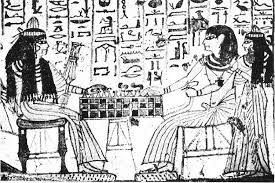
\includegraphics[width=0.8\textwidth]{figs/Senet.jpeg} 
    
    Fonte: {\cite{piccione1980}}.
\end{figure}

Com o avanço da tecnologia e o maior acesso aos meios digitais, a indústria de jogos vem se fortalecendo e crescendo a cada dia. Em 2020, a quantidade de pessoas que jogam regularmente algum tipo de jogo chegou a 3,1 bilhões, representando 40\% da população mundial\footnote{\url{https://www.dfcint.com/dossier/global-video-game-consumer-population/}, acessado em \today.}, sendo utilizada como forma de entretenimento, distração, passatempo e até mesmo como fonte de renda para algumas pessoas. Essa grande popularidade talvez se deva à diversidade de interesses e aos diferentes níveis de complexidade que os jogos oferecem.

Um exemplo disso são os jogos de palavras, um nicho tão antigo quanto os jornais. Tais jogos vêm ganhando destaque nos meios digitais, como é o caso do \textit{Wordle}, que desafia o participante a descobrir uma palavra de cinco letras por meio de feedbacks interativos, o qual evidenciou ainda mais o grande interesse do público por quebra-cabeças linguísticos, sendo inclusive adquirido pelo maior jornal do mundo, o \textit{The New York Times}\footnote{\url{https://www.nytimes.com/2022/01/31/business/media/new-york-times-wordle.html}, acessado em \today.}.

\begin{figure}[H]
    \centering
    
    \label{fig:wordle}
    \caption{Interface do jogo Wordle sendo utilizada em um smartphone}
    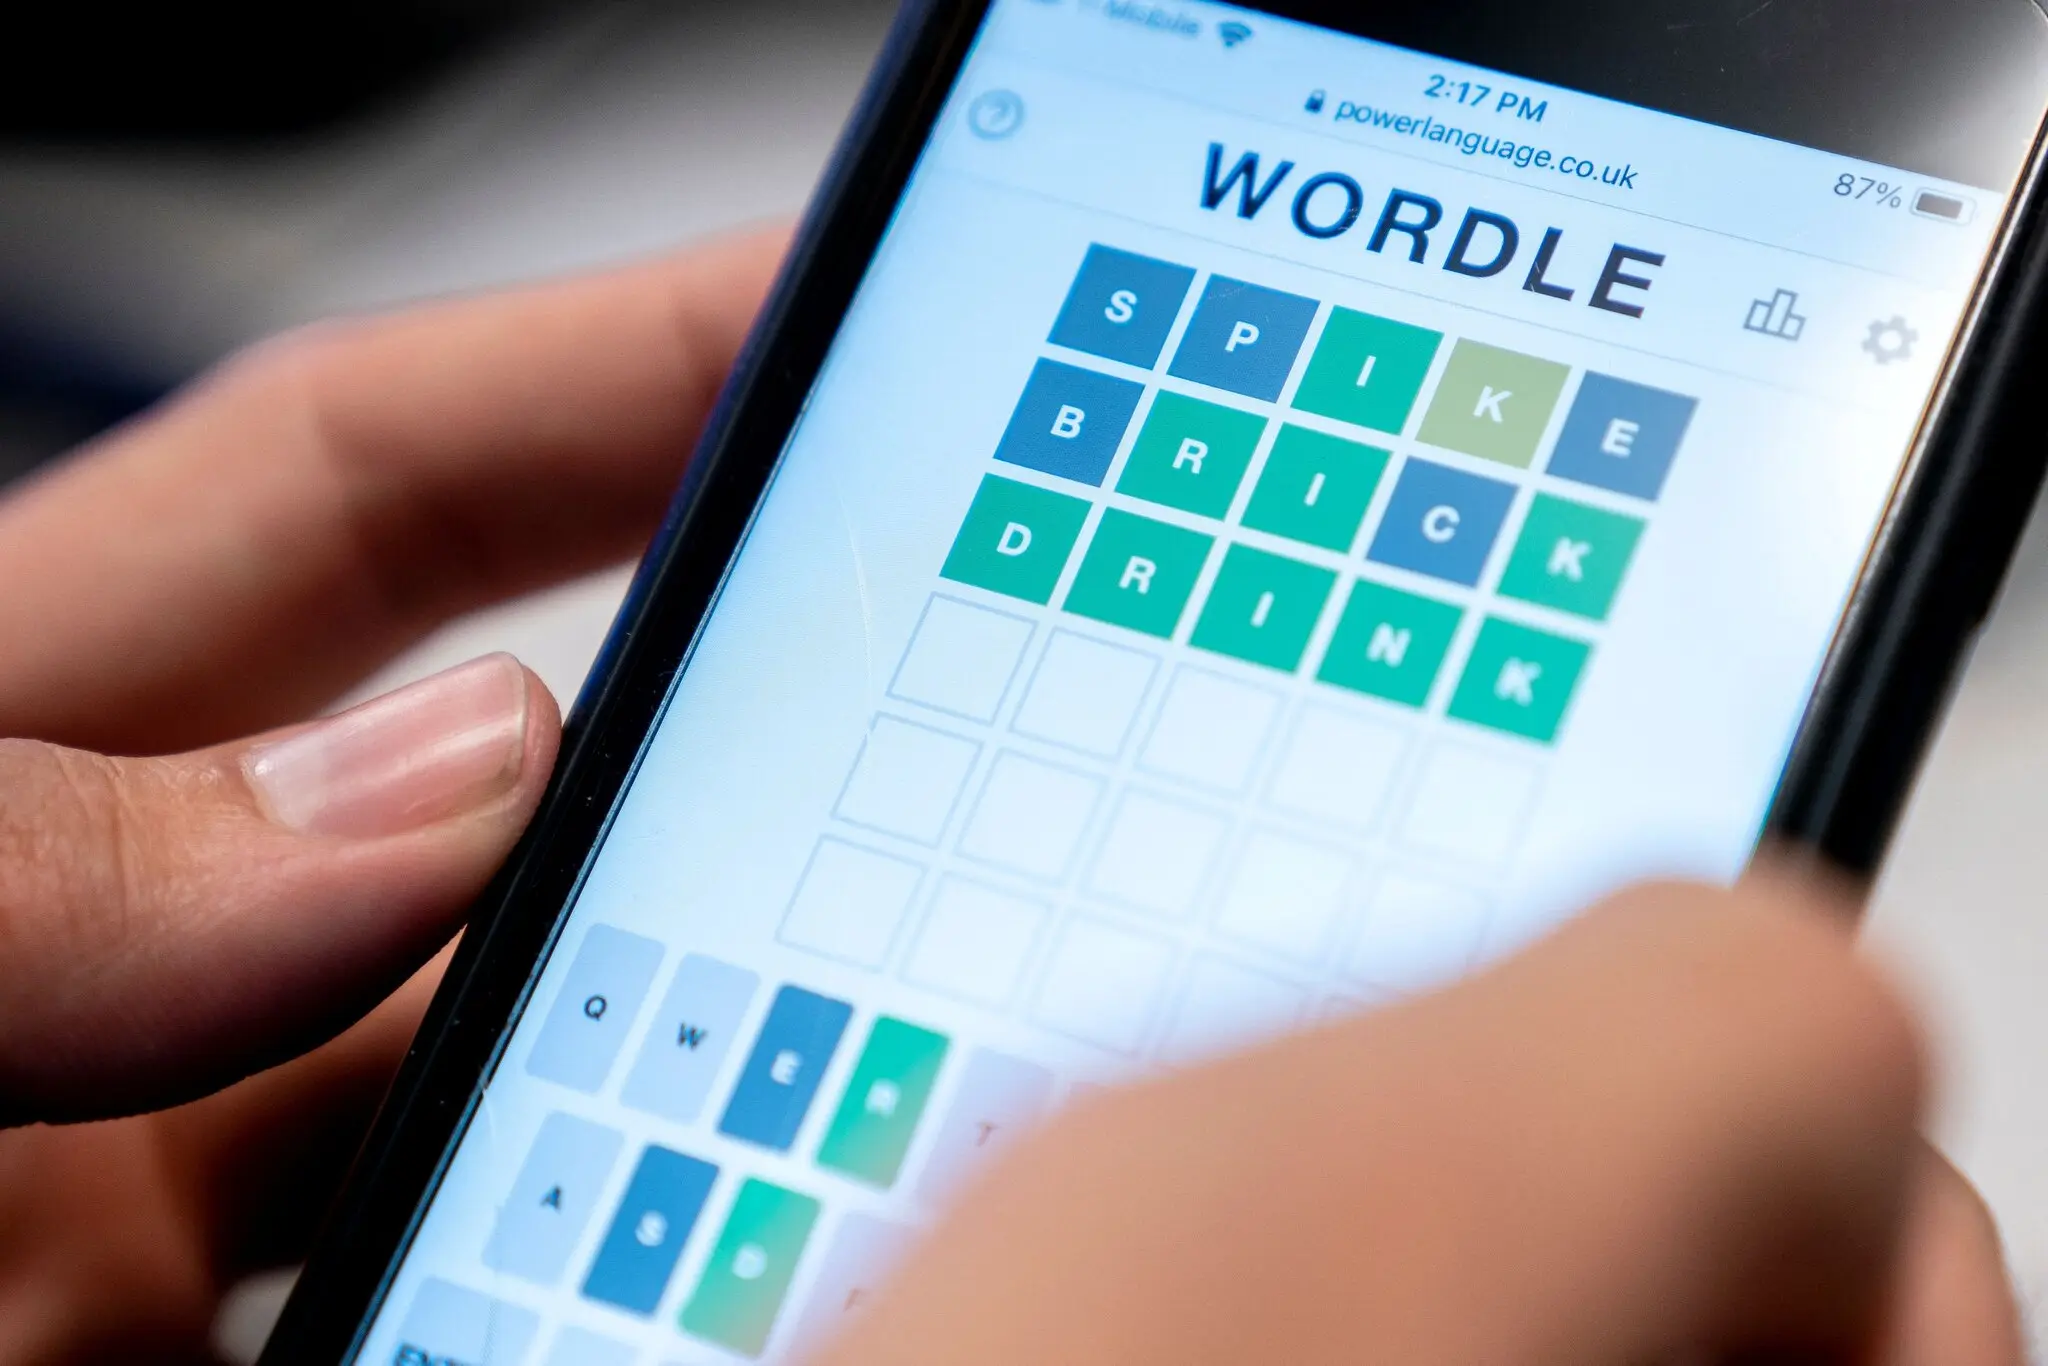
\includegraphics[width=0.8\textwidth]{figs/wordle.png} 
    
   Fonte: \cite{nyt2022wordle}
\end{figure}

Além disso, não é de hoje que grandes jogos passam por transformações significativas com o avanço da tecnologia. O xadrez, jogo de origem milenar e altamente estratégico, tornou-se um marco no campo da Inteligência Artificial (IA), uma vez que foi o primeiro a ser amplamente estudado e "automatizado" em ambientes virtuais. Isso se deu por sua complexidade lógica e previsibilidade de regras, motivo pelo qual foi considerado, durante décadas, o grande desafio da IA.

Nesse contexto, a vitória do computador \textit{Deep Blue}, desenvolvido pela \textit{International Business Machines} (IBM), sobre o campeão mundial Garry Kasparov em 1997 simbolizou um divisor de águas, ao demonstrar a capacidade das máquinas em superar habilidades humanas em tarefas cognitivas complexas \cite{campbell200257}. No entanto, isso não representou algo negativo. Anos após a derrota, o próprio Kasparov afirmou, em uma de suas palestras, que “devemos enfrentar nossos temores se quisermos tirar o máximo proveito da tecnologia... e devemos derrotar esses temores se quisermos tirar o máximo proveito da humanidade” \cite{kasparov2017}, reconhecendo a utilidade da inteligência artificial como ferramenta e destacando que devemos extrair ao máximo suas vantagens.

\begin{figure}[H]
    \centering
    
    \label{fig:kasparovXdeepBlue}
    \caption{Garry Kasparov contra Deep Blue}
    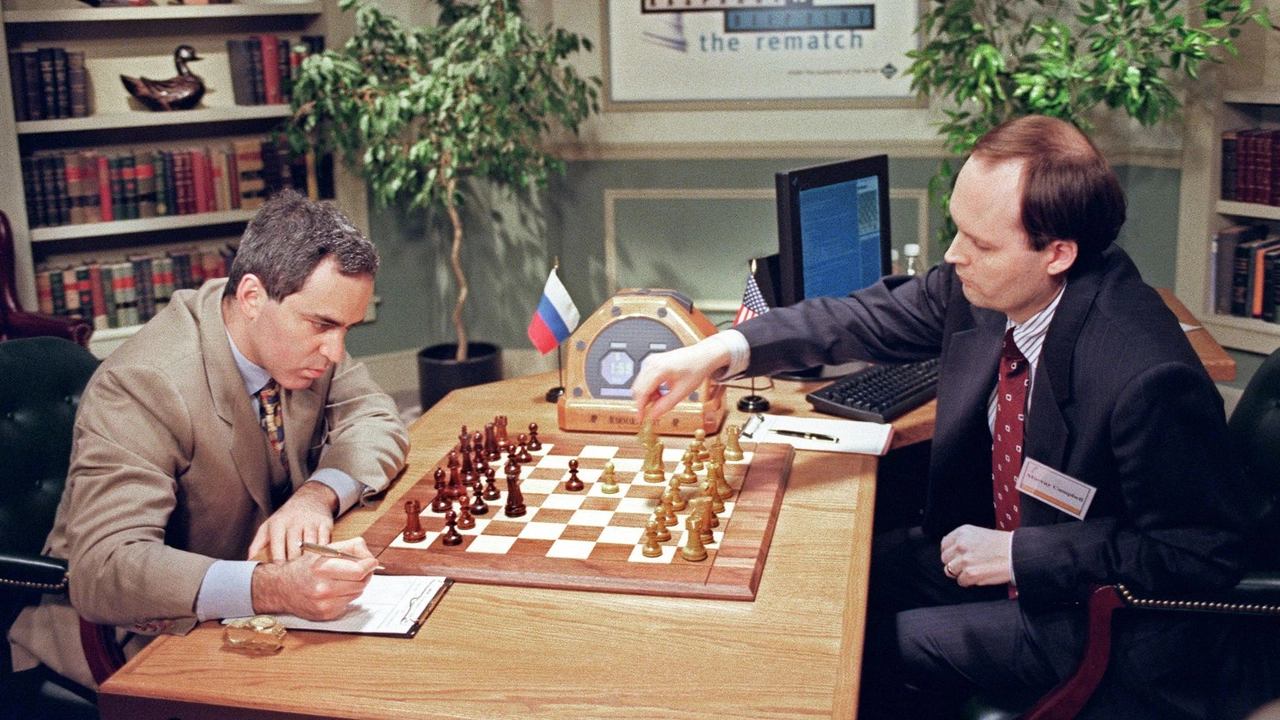
\includegraphics[width=0.8\textwidth]{figs/kasparovXdeepBlue.png} 
    
   Fonte: \cite{aibusiness2022deepblue}
\end{figure}

Com o advento de novas tecnologias, novas modalidades de jogos e desafios passaram a surgir, transformando e recriando clássicos dos jornais. Esses jogos passaram a mesclar inteligência artificial com semântica e exploração linguística, oferecendo novas perspectivas de como jogar. Um exemplo contemporâneo é o \textit{Contexto}\footnote{\url{https://contexto.me}, acessado em \today .}, um jogo online de adivinhação de palavras criado pelo programador Nildo Junior e disponível gratuitamente no navegador.

Inspirado no jogo norte-americano \textit{Semantle}, que utiliza \textit{word embeddings}, uma técnica de processamento de linguagem natural que transforma palavras em vetores numéricos, de forma que palavras com significados semelhantes fiquem próximas entre si no espaço vetorial \cite{mikolov2013efficient}, o Contexto desafia os jogadores a descobrirem a palavra secreta do dia com base em tentativas ilimitadas. A cada palpite, o jogo utiliza um algoritmo de IA para analisar a semelhança contextual entre a palavra sugerida e a palavra secreta, classificando-a em uma posição numérica. A palavra correta ocupa a posição número um, e quanto mais próxima dela estiver a tentativa do jogador, maior será sua pontuação. O sistema também recorre a cores para indicar a proximidade: vermelho para distante, amarelo para moderadamente próximo e verde para muito próximo.

O algoritmo do jogo foi treinado com milhares de textos em português, o que permite identificar palavras utilizadas em contextos semelhantes e calcular a proximidade semântica entre elas. A proposta de oferecer uma nova palavra diariamente incentiva a participação contínua dos jogadores, tornando o Contexto um exemplo atual de como os jogos, desde os tabuleiros do Egito até os navegadores modernos, continuam a evoluir com a tecnologia.

Modelos de IA são amplamente citados em livros, notícias e na literatura acadêmica, sendo utilizados como forma de desafiar o ser humano a ultrapassar seus próprios limites e também como ferramenta para aprimorar o desempenho. Assim, a busca por automatizar a resolução de jogos surge como uma maneira de explorar os limites da IA e, ao mesmo tempo, entender como ela pode nos desafiar. Nesse sentido, este trabalho propõe o desenvolvimento e a avaliação de um sistema automático capaz de resolver partidas do jogo Contexto utilizando modelos de word embeddings.

\section{Problemática}

Com o crescente interesse por jogos linguísticos mediados por IA, como Wordle e Contexto, surge uma nova fronteira de desafios computacionais: compreender o significado das palavras em seu contexto e simular o raciocínio humano na busca pela solução. No entanto, ainda são limitadas as soluções automatizadas eficazes, principalmente em idiomas como o português, que exigem nuances semânticas complexas. Diante disso, a problemática que se apresenta é desenvolver uma abordagem computacional capaz de automatizar a resolução de jogos de adivinhação de palavras em português, levando em consideração os desafios semânticos, contextuais e computacionais inerentes a essa tarefa. 

\section{Justificativa}

O avanço computacional tem possibilitado novas formas de interação homem-máquina, especialmente em domínios que envolvem linguagem natural. Jogos de adivinhação de palavras, como Contexto, têm se destacado por explorar relações semânticas complexas, representando uma oportunidade interessante para testar e aplicar modelos computacionais capazes de simular o raciocínio linguístico humano.

Apesar dos progressos em línguas como o inglês, a automatização desses jogos em português ainda é um campo pouco explorado, principalmente devido à escassez de recursos linguísticos e aos desafios semânticos próprios da língua. Desenvolver uma solução que consiga interpretar contextos, analisar similaridades e encontrar palavras de forma eficiente contribui não apenas para o avanço técnico da área, mas também para o fortalecimento de aplicações educacionais e recreativas com base em IA.

Este trabalho justifica-se pela relevância em propor uma abordagem que integre técnicas de processamento de linguagem natural, com foco na língua portuguesa, promovendo o desenvolvimento de soluções eficientes e adaptadas à nossa realidade linguística.
 
\section{Objetivo}

\subsection{ Objetivo Geral}

% Desenvolver uma abordagem computacional baseada em Inteligência Artificial capaz de automatizar a resolução de jogos de adivinhação de palavras em português, considerando aspectos semânticos, contextuais e computacionais da linguagem natural.

Desenvolver e avaliar um sistema automático capaz de resolver jogos de adivinhação de palavras, utilizando modelos de word embeddings pré-treinados, comparando o desempenho entre eles com base na taxa de acertos e no número de tentativas necessárias.

\subsection{Objetivos Específicos}

Considerando o desenvolvimento do trabalho e o objetivo geral apresentado, destacam-se os seguintes objetivos específicos:

% \begin{itemize}
%     \item Investigar os principais algoritmos e técnicas de \textit{Natural Language Processing} (NLP) aplicáveis à resolução de jogos de palavras;
%     \item Analisar o funcionamento de jogos como \textit{Contexto.me} e \textit{Semantle}, com foco nos critérios de similaridade semântica;
%     \item Implementar um modelo computacional que utilize representações vetoriais de palavras (\textit{word embeddings}) para simular tentativas em jogos de adivinhação;
%     \item Avaliar a eficácia da solução proposta com base na taxa de acertos e no número médio de tentativas;
%     \item Discutir os limites e as possibilidades da aplicação de IA em jogos linguísticos, especialmente no contexto da língua portuguesa.
% \end{itemize}

\begin{itemize}
    \item Desenvolver um sistema para a resolução automática de partidas do jogo Contexto;
    \item Implementar uma heurística de seleção de palavras capaz de conduzir o processo de busca pela palavra secreta;
    \item Avaliar a eficiência da heurística, utilizando métricas como taxa de acertos e número médio de tentativas para mensurar seu desempenho;
    \item Investigar diferentes modelos de word embeddings, compreendendo suas características e abordagens conceituais.
    \item Desenvolver um sistema que permita comparar o desempenho dos diferentes modelos de embeddings sob uma mesma heurística, garantindo uma análise comparativa consistente.
\end{itemize}

\section{Metodologia}

Para este trabalho, adotou-se o método de pesquisa exploratória, pois esse tipo de estudo visa proporcionar maior familiaridade com o problema, tornando-o mais explícito e auxiliando na formulação de hipóteses. O objetivo central da pesquisa é o aprimoramento de ideias ou a descoberta de novas intuições, sendo seu planejamento caracterizado por flexibilidade, o que permite a consideração de diferentes aspectos relacionados ao fenômeno estudado.

As pesquisas exploratórias normalmente envolvem levantamento bibliográfico, análise de exemplos que ampliem a compreensão do tema e entrevistas com especialistas na área. Neste trabalho, optou-se por concentrar a análise principalmente em fontes bibliográficas e exemplos relevantes, em conformidade com os objetivos da pesquisa e com a natureza exploratória do estudo.


\section{Organização}
O presente trabalho está organizado da seguinte forma:

O \textbf{Capítulo 1} apresenta a introdução do estudo, contextualizando o problema de pesquisa, sua relevância no cenário atual, os objetivos gerais e específicos, bem como a metodologia empregada.

O \textbf{Capítulo 2} trata dos trabalhos relacionados, reunindo estudos e projetos previamente desenvolvidos que possuem afinidade com o tema abordado, a fim de embasar teoricamente a proposta.

O \textbf{Capítulo 3} aborda os principais conceitos, fundamentos e ferramentas envolvidos na execução do projeto, detalhando os elementos que sustentam a construção da proposta.

O \textbf{Capítulo 4} descreve o desenvolvimento da solução proposta, detalhando as etapas e processos adotados na implementação e na construção da resolução de jogos de adivinhar palavras.

O \textbf{Capítulo 5} apresenta as considerações finais, destacando os resultados obtidos, as contribuições do trabalho e sugestões para futuras melhorias e desdobramentos do projeto.